\documentclass{standalone}
\usepackage{xstring}
\usepackage{tikz}
\usetikzlibrary{calc, decorations.pathreplacing, calligraphy}
\usepackage{xifthen}
\usepackage{amsmath}
\usetikzlibrary{bayesnet}

\newcommand{\Height}{0.8cm}% Adjust size of square as desired
\newcommand{\Width}{1.6cm}% Adjust size of square as desired

\tikzset{GreySquare/.style={
    inner sep=0pt,
    text width=\Width,
    minimum size=\Height,
    draw=black,
    fill=black!20,
    align=center
    }
}
\tikzset{LightGreySquare/.style={
    inner sep=0pt,
    text width=\Width,
    minimum size=\Height,
    draw=black,
    fill=black!5,
    align=center
    }
}

\tikzset{GreenSquare/.style={
    inner sep=0pt,
    text width=\Width,
    minimum size=\Height,
    draw=black,
    fill=green!15,
    align=center
    }
}
\tikzset{DarkGreenSquare/.style={
    inner sep=0pt,
    text width=\Width,
    minimum size=\Height,
    draw=black,
    fill=green!50,
    align=center
    }
}
\tikzset{RedSquare/.style={
    inner sep=0pt,
    text width=\Width,
    minimum size=\Height,
    draw=black,
    fill=red!15,
    align=center
    }
}
\tikzset{DarkRedSquare/.style={
    inner sep=0pt,
    text width=\Width,
    minimum size=\Height,
    draw=black,
    fill=red!50,
    align=center
    }
}
\tikzset{BlueSquare/.style={
    inner sep=0pt,
    text width=\Width,
    minimum size=\Height,
    draw=black,
    fill=blue!15,
    align=center
    }
}
\tikzset{DarkBlueSquare/.style={
    inner sep=0pt,
    text width=\Width,
    minimum size=\Height,
    draw=black,
    fill=blue!50,
    align=center
    }
}
\tikzset{Red2Square/.style={
    inner sep=0pt,
    text width=\Width,
    minimum size=\Height,
    draw=black,
    fill=orange!25,
    align=center
    }
}
\tikzset{DarkRed2Square/.style={
    inner sep=0pt,
    text width=\Width,
    minimum size=\Height,
    draw=black,
    fill=orange!70,
    align=center
    }
}
\tikzset{Blue2Square/.style={
    inner sep=0pt,
    text width=\Width,
    minimum size=\Height,
    draw=black,
    fill=yellow!25,
    align=center
    }
}
\tikzset{DarkBlue2Square/.style={
    inner sep=0pt,
    text width=\Width,
    minimum size=\Height,
    draw=black,
    fill=yellow!70,
    align=center
    }
}
\tikzset{Square/.style={
    inner sep=0pt,
    text width=\Width,
    minimum size=\Height,
    draw=black,
    fill=red!0,
    align=center
    }
}

\begin{document}

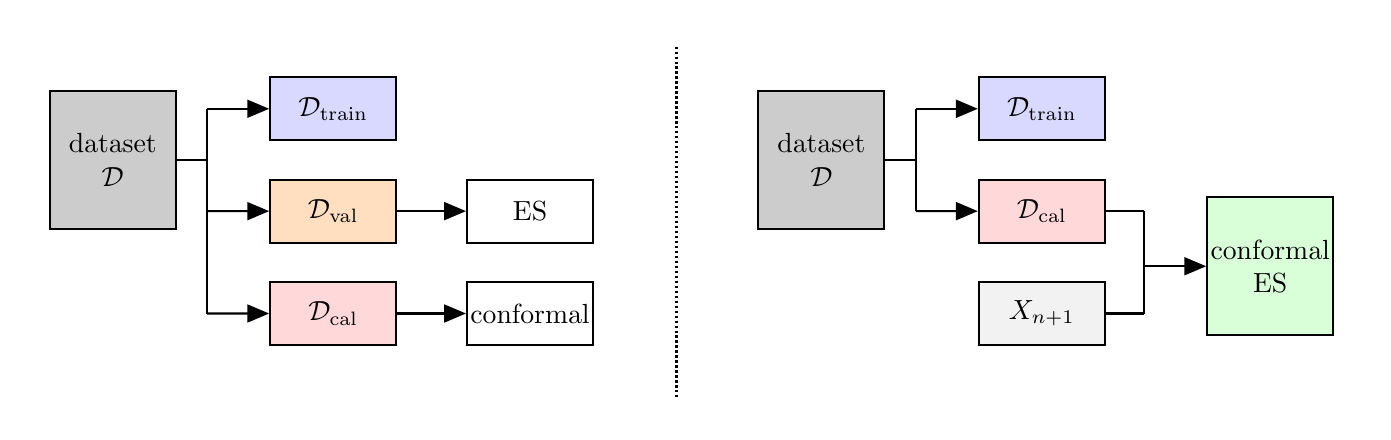
\begin{tikzpicture}[draw=black, thick, x=\Width,y=\Height]
    \useasboundingbox (-6.3,-1.5) rectangle (4.3,4.6);
    
    \node (D)[GreySquare, minimum height = 1.75cm] at (0,2.5) {dataset \\ $\mathcal{D}$};
    
    \node (Dtrain) [BlueSquare, right of=D, xshift=1.8cm, yshift=0.65cm] {$\mathcal{D}_{\text{train}}$};
    
    \node (Dcal) [RedSquare, below of=Dtrain, yshift=-0.3cm] {$\mathcal{D}_{\text{cal}}$};
     
    \coordinate [right of=D, xshift=0.2cm] (s1);
        \draw (D.east) -- (s1);
    \coordinate [above of=s1, yshift=-0.35cm] (s2);
    \coordinate [below of=s1, yshift=0.35cm] (s3);
        \draw (s1) -- (s3);
        \draw (s1) -- (s2);
        \draw [->] (s2) -- (Dtrain.west);
        \draw [->] (s3) -- (Dcal.west);
    
    
    \node (Dtest) [LightGreySquare, below of=Dcal, yshift=-0.3cm] {$X_{n+1}$};
    \coordinate [right of=Dcal, xshift=0.3cm] (s4);
    \coordinate [right of=Dtest, xshift=0.3cm] (s5);
        \draw (Dcal) -- (s4);
        \draw (Dtest) -- (s5);
    \coordinate [below of=s4, yshift=0.3cm] (s6);
        \draw (s4) -- (s5);
    
    \node (es) [GreenSquare, minimum height = 1.75cm, right of=s6, xshift=0.6cm]
    {conformal\\ES};
        \draw [->] (s6) -- (es.west);
        
        
    \node (D_old)[GreySquare, minimum height = 1.75cm, left of=D, xshift=-8cm] {dataset \\ $\mathcal{D}$};
    
    \node (Dtrain_old) [BlueSquare, right of=D_old, xshift=1.8cm, yshift=0.65cm] {$\mathcal{D}_{\text{train}}$};
    
    \node (Dval_old) [Red2Square, below of=Dtrain_old, yshift=-0.3cm] {$\mathcal{D}_{\text{val}}$};
    
    \node (Dcal_old) [RedSquare, below of=Dval_old, yshift=-0.3cm] {$\mathcal{D}_{\text{cal}}$};
    
    \coordinate [right of=D_old, xshift=0.2cm] (c1);
        \draw (D_old.east) -- (c1);
    \coordinate [above of=c1, yshift=-0.35cm] (c2);
    \coordinate [below of=c1, yshift=0.35cm] (c3);
        \draw (c1) -- (c3);
        \draw (c1) -- (c2);
        \draw [->] (c2) -- (Dtrain_old.west);
        \draw [->] (c3) -- (Dval_old.west);
    \coordinate [below of=c3, yshift=-0.3cm] (c4);
        \draw [->] (c4) -- (Dcal_old.west);
        \draw (c3) -- (c4);
    
    \node (es) [Square, right of=Dval_old, xshift=1.5cm]{ES};
    \node (conformal) [Square, right of=Dcal_old, xshift=1.5cm]{conformal};
        \draw [->] (Dval_old.east) -- (es.west);
        \draw [->] (Dcal_old.east) -- (conformal.west);
        
    
    \coordinate (l1) at (-1.15,4.3);
    \coordinate (l2) at (-1.15,-1.3);
    \draw[densely dotted] (l1) -- (l2);

        


    
    
\end{tikzpicture}


\end{document}